\documentclass[10pt]{article}

\usepackage[T1]{fontenc}
\usepackage[utf8]{inputenc}
%\usepackage{beton}
%\usepackage{ccfonts}
%\usepackage{concrete}
\usepackage{concmath}
\usepackage{eulervm}
\usepackage{amsmath,amsthm,amssymb}
\usepackage{mathtools}
\usepackage{multicol}
\usepackage{marginnote}
\usepackage{pgfplots}
\usepackage{float}
\usepackage{hyperref}
\usepackage{bbm}
\usepackage{booktabs}
\usepackage{xcolor-solarized}
\usepackage{xcolor}
\pgfplotsset{compat=1.5}

\usepackage{listings}
\usepackage{xcolor}
\definecolor{codegreen}{rgb}{0,0.6,0}
\definecolor{codegray}{rgb}{0.5,0.5,0.5}
\definecolor{codepurple}{rgb}{0.58,0,0.82}
\definecolor{backcolour}{rgb}{0.95,0.95,0.92}
\lstdefinestyle{mystyle}{
    backgroundcolor=\color{backcolour},   
    commentstyle=\color{codegreen},
    keywordstyle=\color{magenta},
    numberstyle=\tiny\color{codegray},
    stringstyle=\color{codepurple},
    basicstyle=\ttfamily\footnotesize,
    breakatwhitespace=false,         
    breaklines=true,                 
    captionpos=b,                    
    keepspaces=true,                 
    numbers=left,                    
    numbersep=5pt,                  
    showspaces=false,                
    showstringspaces=false,
    showtabs=false,                  
    tabsize=2
}

\lstset{language=Python, style=mystyle}

\usepackage{mathtools}

\usepackage{wasysym}
\usepackage[margin=1.5in]{geometry} 
\usepackage{enumerate}
\index{\usepackage}\usepackage{multicol}

\newcommand{\N}{\mathbf{N}}
\newcommand{\Z}{\mathbb{Z}}

\newcommand{\R}{\mathbf{R}}
\newcommand{\C}{\mathbf{C}}
\newcommand{\Pbb}{\mathbb{P}}
\newcommand{\Fcal}{\mathcal{F}}
\newcommand{\Lcal}{\mathcal{L}}
\newcommand{\Acal}{\mathcal{A}}
\newcommand{\Ecal}{\mathcal{E}}
\newcommand{\Ebb}{\mathbb{E}}
\newcommand{\Qbb}{\mathbb{Q}}


\renewcommand{\mathbf}{\mathbold}

\newenvironment{theorem}[2][Theorem]{\begin{trivlist}
  \item[\hskip \labelsep {\bfseries #1}\hskip \labelsep {\bfseries #2.}]}{\end{trivlist}}
\newenvironment{lemma}[2][Lemma]{\begin{trivlist}
  \item[\hskip \labelsep {\bfseries #1}\hskip \labelsep {\bfseries #2.}]}{\end{trivlist}}
\newenvironment{exercise}[2][Exercise]{\begin{trivlist}
  \item[\hskip \labelsep {\bfseries #1}\hskip \labelsep {\bfseries #2.}]}{\end{trivlist}}
\newenvironment{reflection}[2][Reflection]{\begin{trivlist}
  \item[\hskip \labelsep {\bfseries #1}\hskip \labelsep {\bfseries #2.}]}{\end{trivlist}}
\newenvironment{proposition}[2][Proposition]{\begin{trivlist}
  \item[\hskip \labelsep {\bfseries #1}\hskip \labelsep {\bfseries #2.}]}{\end{trivlist}}
\newenvironment{corollary}[2][Corollary]{\begin{trivlist}
  \item[\hskip \labelsep {\bfseries #1}\hskip \labelsep {\bfseries #2.}]}{\end{trivlist}}

\newenvironment{definition}[2][Definition]{\begin{trivlist}
  \item[\hskip \labelsep {\bfseries #1}\hskip \labelsep {\bfseries #2.}]}{\end{trivlist}}

\definecolor{solar}{rgb}{0.9960, 0.9960, 0.9647}

\begin{document}
  \pagecolor{solar}
	
  \renewcommand{\qedsymbol}{\smiley}
	\title{Investments Class \\ Problem set 8}
	\author{Daniel Grosu, William Martin, Denis Steffen}
		
\maketitle

\begin{exercise}{1}(CAPM)
\end{exercise}
\begin{itemize}
  \item[(a)] By definition of the beta of an asset, we have: $$ \sigma_M^2 = \frac{Cov(r_A,r_M)}{\beta_A} = \frac{Corr(r_A,r_M)\sigma_M\sigma_A}{\beta_A}$$ and so $$ \sigma_M = \frac{Corr(r_A,r_M)\sigma_A}{\beta_A} = 0.2$$
  Thus we can deduce the beta of asset B: $$\beta_B = \frac{Corr(r_B,r_M)\sigma_M\sigma_B}{\sigma_M^2} = 0.75$$
  And, 
  $$Corr(r_C,r_M) = \frac{Cov(r_C,r_M)}{\sigma_C\sigma_M} = \frac{\beta_C\sigma_M}{\sigma_C}  = 0.8$$
  \item[(b)] Assuming the CAPM holds, we can know compute the market portfolio return using asset A: 
  $$ r_A = r_0 + \beta_A(r_M-r_0) \quad \Rightarrow \quad r_M = \frac{r_A-r_0}{\beta_A} + r_0 = 0.06$$ 
  And using the CAPM formula for assets B and C, we obtain: $ r_B = 0.05$ and $r_C = 0.076$.
  \item[(c)] We can see that asset D has a better expected return than all assets A, B and C, but has a lower standard deviation than C. So the security D will be over the market security line and is undervalued as it has greater return for less risk than C (that is on the line). 
  
  The alpha of D is in the following equation: 
  $$ r_D - r_0 = \alpha_D + \beta_D(r_M-r_0) \quad \Rightarrow \quad \alpha_D = r_D^e -\beta_D*r_M^e = 0.06 - 0.048 = 0.012.$$ 
  The systematic risk is given by: $\beta_D^2\sigma_M^2 = 0.0576$, and the residual risk equals the standard deviation minus the systematic risk: $\sigma_D^2-\beta_D^2\sigma_M^2 = 0.0208.$

  In addition, the Information Ratio is the ratio $IR = \frac{\alpha_D}{\sigma_D} =\frac{0.012}{0.08}= 0.15$
  \item[(d)] Finally, the optimal portfolio with risk-aversion $1$ is given by:
  $$ w = \Sigma^{-1}(\mu-r_0\mathbbm{1}_5)$$ with assets (A,B,C,M,D), $\mu = (r_A,r_B,r_C,r_M,r_D)^\top = (0.032,0.05,0.076,0.06,0.08)^\top$. So the covariance matrix $\Sigma$ is: 
  $$ \Sigma = \left[\begin{array}{ccccc}
    \sigma_A^2& 0 &0 &Cov(r_A,r_M)& 0\\
    0&\sigma_B^2 & 0 & Cov(r_B,r_M)&0 \\
    0&0&\sigma_C^2&Cov(r_C,r_M)&0\\
    Cov(r_A,r_M)&Cov(r_B,r_M)&Cov(r_C,r_M)&\sigma_M^2&Cov(r_D,r_M)\\
    0&0&0&Cov(r_D,r_M)&\sigma_D^2
  \end{array}\right]$$ 
  And with the given parameters: 
  $$ \Sigma = \left[\begin{array}{ccccc}
    0.0225 & 0 & 0 & 0.012 &0 \\
    0 & 0.0625 & 0 & 0.03 & 0 \\
    0 & 0 & 0.1225 & 0.056 & 0 \\
    0.012 & 0.03 & 0.056 & 0.04 & 0.048 \\
    0 & 0 & 0 & 0.048 & 0.0784 
  \end{array}\right]$$

  And the optimal portfolio weights are: 
 $$ w = (0.3562, -0.7581, 0.3392, 0.2579, 0.6074)$$
 The weight invested in the T-bills, that are our riskfree asset, is $w_0 = 1- \mathbbm{1}'w = 0.1974$.

 Now, we can compute the usual statistics for this portfolio. First, the expected return is $w'\mu + w_0r_0 = 0.0673$ and the standard deviation equals $\sqrt{w'\Sigma w} = 0.2175$. And the Sharpe Ratio is $ \frac{w'\mu - r_0}{\sqrt{w'\Sigma w}} = 0.2175$.
\end{itemize}
  
\newpage

\begin{exercise}{2}{The momentum factor}
\end{exercise}

After creating 10 portfolios sorted by average return computed as described in the problems et sheet, we compute the value-weighted  returns  of these portfolios. We then create a zero-cost portfolio which consists  in going long in the decile with the highest pas returns and shorting the decile with the lowest past return. Plotting the returns of this newly created portfolio gives us figure \ref{ps8_ex2_plot1}.

\begin{figure}[h]
    \centering
    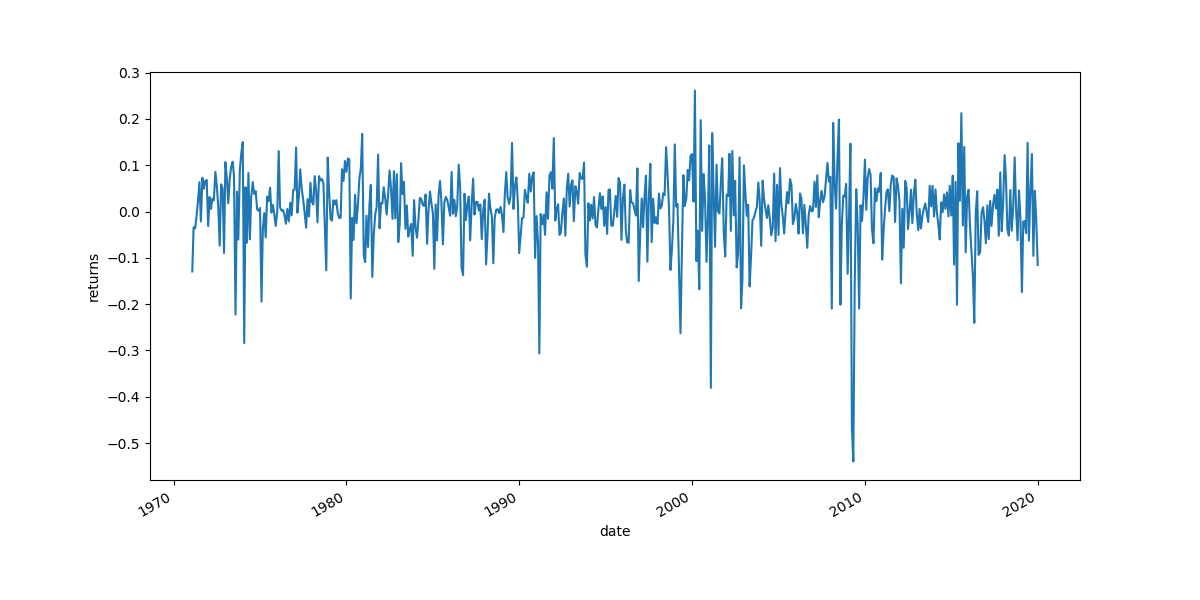
\includegraphics[scale=0.5]{ps8_ex2_plot1.png}
    \caption{Returns of a zero-cost portfolio going  long on highest pas returns and shorting lowest past returns}
    \label{ps8_ex2_plot1}    
\end{figure}

We then run the following regressions, similarly as in problem set 5 (the zero-cost strategy is denoted $ZC$):

\begin{align*}	
	R_{ZC} &= \alpha_a +  \beta_1 R^e_{mt} + \beta_2 SMB + \beta_3 HML \\
	R_{ZC}  &= \alpha_b + \beta_1 R^e_{mt} + \beta_2 SMB + \beta_3 HML + \beta_4 MOM
\end{align*}  

Where the $SMB$ and $HML$ factors are factors from Kenneth French’s website. $MOM$ is the momentum factor. Moreover, returns denotes $R^e$ are excess returns. We obtain $\alpha_{a} = 0.00985$ and $\alpha_{b} = -0.00378$.   
   
\bigbreak

We now create 2 portfolios based on the previous month's market capitalization.  The zero-cost strategy's return is given in figure \ref{ps8_ex2_plot2}.

\begin{figure}[h]
    \centering
    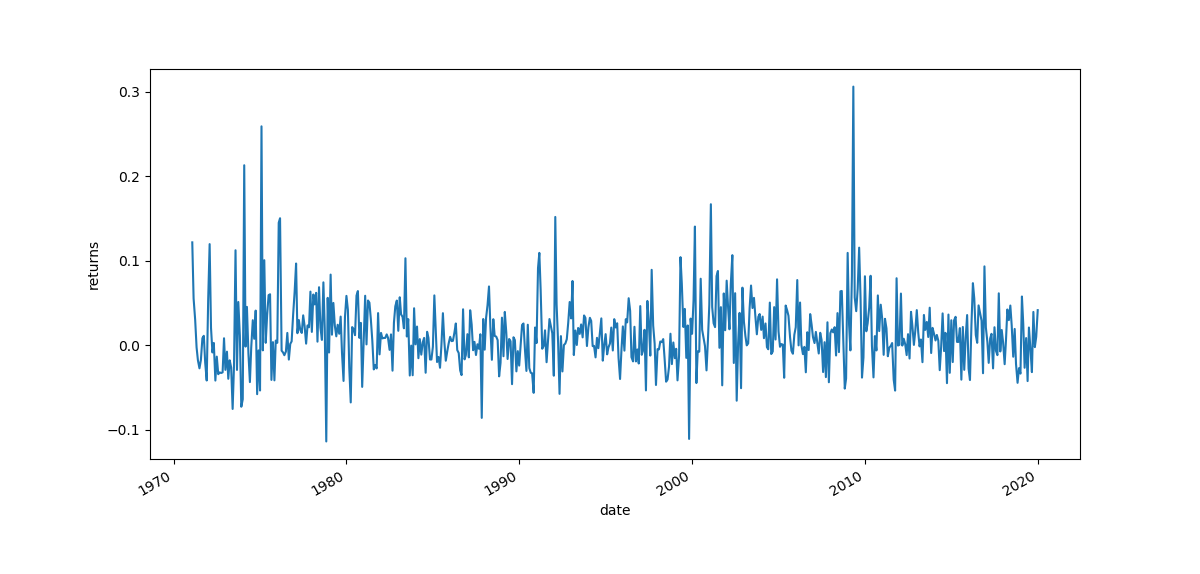
\includegraphics[scale=0.5]{ps8_ex2_plot2.png}
    \caption{Returns of a zero-cost portfolio going  long on highest pas returns and shorting lowest past returns}
    \label{ps8_ex2_plot2}    
\end{figure}

We now run the same regressions:

\begin{align*}	
	R_{ZC} &= \alpha_c +  \beta_1 R^e_{mt}  + \beta_2 SMB + \beta_3 HML \\
	R_{ZC}  &= \alpha_d + \beta_1 R^e_{mt} + \beta_2 SMB + \beta_3 HML + \beta_4 MOM
\end{align*}  

We obtain $\alpha_{c} =  -0.00960$ and $\alpha_{d} = -0.01151$.
   
\end{document}



\appendix

